\documentclass[]{style/ceurart}
\sloppy

\usepackage{listings}
\lstset{breaklines=true}
\usepackage{graphicx}

\begin{document}

\copyrightyear{2024}
\copyrightclause{Copyright for this paper by its authors.
  Use permitted under Creative Commons License Attribution 4.0
  International (CC BY 4.0).}

\conference{CLEF 2024: Conference and Labs of the Evaluation Forum, September 9-12, 2023, Grenoble, France}

\title{Tiled Raster Compression and Embeddings for Multilabel Classification in GeoLifeCLEF 2024}

\author[1]{Anthony Miyaguchi}[
orcid=0000-0002-9165-8718,
email=acmiyaguchi@gatech.edu,
]
\cormark[1]
\author[1]{Patcharapong Aphiwetsa}[
email=paphiwetsa3@gatech.edu,
]
\author[1]{Mark McDuffie}[
email=mmcduffie8@gatech.edu,
]

\address[1]{Georgia Institute of Technology, North Ave NW, Atlanta, GA 30332}
\cortext[1]{Corresponding author.}

\begin{abstract}
In this paper, we explore methods to solve the multilabel classification task posed by the GeoLifeCLEF 2024 competition, which aims to predict the presence and absence of plant species at specific locations using spatial and temporal remote sensing data. 
Our approach focuses on data preprocessing and the application of various modeling techniques to handle the sparse label space and computational challenges. 
We employ unsupervised methods to build valuable data representations and experiment with several classical and neural network-based models.
\end{abstract}

\begin{keywords}
  GeoLifeCLEF,
  remote sensing,
  contrastive learning,
  multi-label classification
\end{keywords}


\maketitle

\section{Introduction}

GeoLifeCLEF is a task organized within the LifeCLEF lab at the CLEF 2024 conference. 
GeoLifeCLEF aims to predict what plant species are present and absent at a specific location given spatial and temporal remote sensing data. 
Modeling species density distributions can be helpful in biodiversity management and conservation, among other things.

In this project, we explore methods to solve the posed multi-label classification task and try to incorporate unsupervised methods for building valuable representations from the data. 
Much of the work was focused on pre-processing the data from the competition for modeling and experimenting with various modeling approaches to deal with computational challenges related to the sparse label space.

\section{Dataset and Evaluation}

The competition has three major components. 
The first are the metadata associated with the competition comprising a presence-only training, presence-absence training, and presence-absence test set. 
The metadata provides a mapping between location and the species labels available for supervised training. 
The second are the remote-sensing and raster data provided in pixel format. 
The final component is time series data containing quarterly environmental data over a 20 year period. 

The presence-only training dataset comprises 5M examples over 4M survey sites distributed across Western Europe.
The presence-absent dataset data of a similar schema, but the semantics are stricter -- species not included in the survey are known to be absent. 
This is not necessarily the case with the present-only data since they are scraped from crowd-sourced data, meaning there may be gaps in reported species. 
The datasets include an identifier for the survey site and the latitude and longitude. 
We compute a projection into EPSG 3035, which allows for Euclidean distance in units of meters. 

\begin{table}[ht]
\centering
\caption{Number of survey identifiers per dataset.}
\label{lst:counts}
\begin{tabular}{|c|c|}
\hline
dataset   & count   \\ \hline
po        & 5079797 \\ \hline
pa\_train & 1483637 \\ \hline
pa\_test  & 4716    \\ \hline
\end{tabular}
\end{table}

\begin{lstlisting}[caption={Schema of the metadata.}, captionpos=b,label={lst:schema},frame=single]
  |-- dataset: string (nullable = true)
  |-- surveyId: integer (nullable = true)
  |-- lat_proj: double (nullable = true)
  |-- lon_proj: double (nullable = true)
  |-- lat: double (nullable = true)
  |-- lon: double (nullable = true)
  |-- year: integer (nullable = true)
  |-- geoUncertaintyInM: double (nullable = true)
  |-- speciesId: double (nullable = true) 
\end{lstlisting}

The raster and satellite imagery accounts for the majority of the available data. 
We are provided GeoTIFF files for various measures such as elevation, roads, population, and soil. 
The GeoTIFF files are bounded by a GeoJSON polygon that covers Western Europe. 
RGB-NIR satellite imagery is provided directly as tiles associated with each survey site.

\begin{figure}
\begin{lstlisting}[frame=single]
  {
    "type": "Polygon",
    "coordinates": [
        [
            [-32.26344, 26.63842],
            [-32.26344, 72.18392],
            [35.58677, 72.18392],
            [35.58677, 26.63842],
            [-32.26344, 26.63842],
        ]
    ],
}
\end{lstlisting}
\caption{GeoJSON polygon for region specified by GeoLifeCLEF 2024.}
\label{lst:polygon}
\end{figure}

\subsection{Processing Raster Data}

We process GeoTIFF files for use within a supervised learning process. 
There is significant in-memory overhead with tiling the data since we need to store the 128x128 byte array for each survey site. 
We fork the official \texttt{plantnet/GeoLifeCLEF} data loaders to pre-compute tiles for each of the provided GeoTIFF under 1GB. 
Certain rasters do not fit into memory (e.g., elevation raster at 11GB); therefore, we omit them from our experiments. 
We only compute the tiles associated with the survey identifiers in our metadata, which helps limit the size of the resulting dataset. 
In addition to generating tiled images, we compute the 2D-DCT on the resulting tile images and keep low-frequency coefficients as features in downstream modeling. 


\begin{figure}[h!]
    \centering
    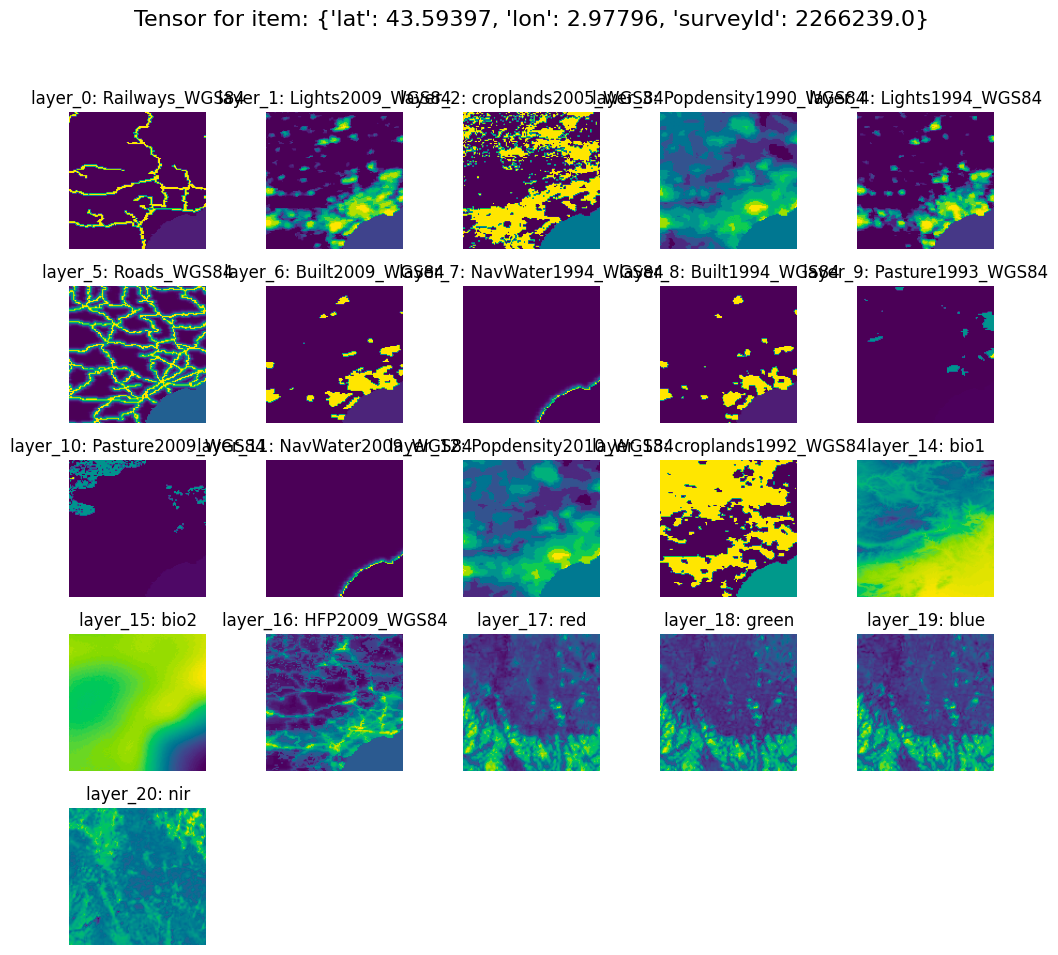
\includegraphics[width=0.9\textwidth]{figures/tiled-raster.png}
    \caption{
        Example of a tiled raster image. 
        The image is a 128x128 tile of the RGB-NIR satellite imagery. 
        The image is associated with a survey site and is used as input to the model. 
    }
    \label{fig:tiled-raster}
\end{figure}

We implement a wrapper around the ND-DCT that we can use in Spark. 
While we can access a native 1D-DCT implementation for feature pre-processing, we lose significant spatial information if we flatten the image and run a low-pass filter as seen in figure \ref{fig:dct-lowpass}.

% three images side by side
\begin{figure}
  \centering
  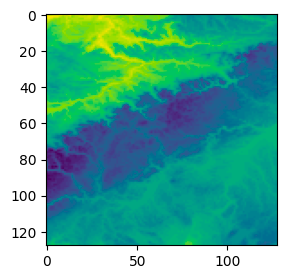
\includegraphics[width=0.3\textwidth]{figures/dct-original.png}
  \hfill
  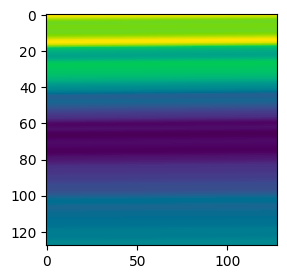
\includegraphics[width=0.3\textwidth]{figures/dct-1d-lowpass.png}
  \hfill
  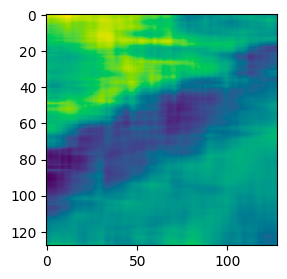
\includegraphics[width=0.3\textwidth]{figures/dct-2d-lowpass.png}
  \caption{
    Example of low-pass filtering using the DCT.
    (a) Original bio1 raster image.
    (b) Low-pass filter using the first 50 coefficients of the 1D-DCT, reshaping on the first axis (row-major order).
    (c) Low-pass filter using the 2D-DCT using the top-left 8x8 coefficients.
  }
  \label{fig:dct-lowpass}
\end{figure}

\subsection{Processing Time-Series Data}

In addition to the raster data, we process time series data so they fit within our modeling framework.
We have access to quarterly time-series data for each survey site over 20 years.
Some sites have missing data, which we pad with zeros.
We compute the 1D DCT on the time series data and keep the low-frequency coefficients as features in downstream modeling.
We keep the first 64 coefficients in the transformed space, which we choose to parallel with the 8x8 2D-DCT coefficients extracted from the raster data.
As shown in Figure \ref{fig:dct-timeseries}, the original time-series data and its DCT are displayed side by side.


% two images side by side
\begin{figure}[h!]
  \centering
  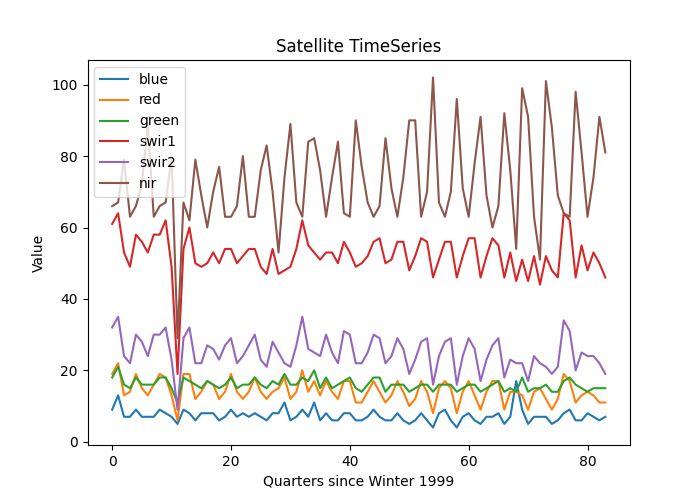
\includegraphics[width=0.495\textwidth]{figures/6-bands.png}
  \hfill
  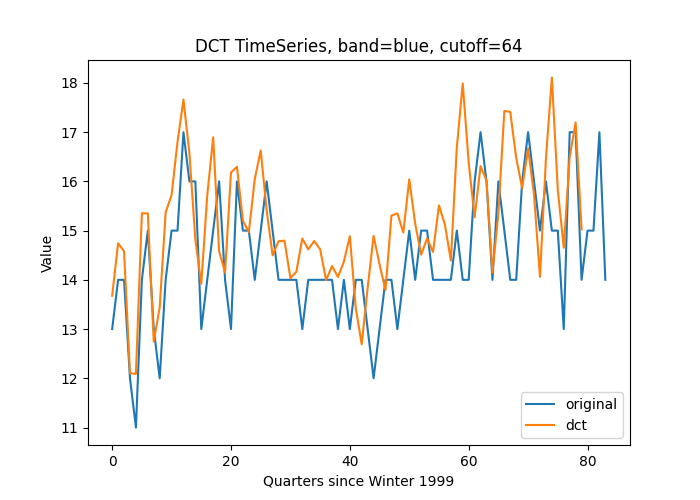
\includegraphics[width=0.495\textwidth]{figures/both.png}
  \caption{
    Example of time-series data and its DCT.
    (a) Original time-series data.
    (b) Blue band time-series approximated using DCT.
  }
  \label{fig:dct-timeseries}
\end{figure}
\subsection{Raster Data Augmentation}

We apply augmentations to our data to encourage model invariance to rotation and reflection.
We can implement augmenting transforms in pixel space by rotating and flipping images before sending them into a model.
Equivalent augmentations exist in frequency space.
For example, a 90-degree rotation in pixel space is equivalent to the transpose of the 2D-DCT coefficients.
We can flip the image in pixel space by alternating the signs of the 2D-DCT coefficients along a given axis.
Rotations and flips along the axis give us enough flexibility to implement useful symmetries in the data to improve generalization.

\begin{figure}
\begin{lstlisting}[language=Python,frame=single]
class DCTHorizontalFlip:
    def __init__(self, k=8):
        self.odd_factor = -torch.ones((k, k))
        for i in range(0, k, 2):
            self.odd_factor[i, :] = 1

    def forward(self, X):
        return X * self.odd_factor
\end{lstlisting}
\caption{Augmentation of 2D-DCT coefficients.}
\label{lst:augmentation}
\end{figure}
\section{Experiments}

We explore several solutions for the multi-label classification problem. 
We use Luigi \cite{Rouhani2024spotify} as our workflow management tool, which is easy to set up and provides idempotent directed acyclic graphs (DAGs) of tasks. 
We use Spark \cite{armbrust2015spark} to perform data extraction, transformation, and loading (ETL) from tarred images and CSV files to columnar parquet files. 

\subsection{Naive Multi-class Classification}

Our first goal is to learn the relationship between geospatial features (latitude and longitude) and the species labels. 
Our first model is to learn a linear relationship between the features and response using a logistic regression to put together a simple baseline. 
This numerically simple model can be learned using Spark via stochastic gradient descent (SGD). 
As a validation, we build a model using the top 10 species by frequency. 
We obtain an accuracy of 0.09, which is better than random but roughly equivalent to always choosing the most frequent species.

We immediately run into computational issues when we scale up the process to use all 5 million rows and 10,358 species. 
We quickly run into out-of-memory (OOM) issues when we try to fit a logistic regression model using scikit-learn or statsmodels.
When we run the same procedure in Spark, we can configure a model that takes advantage of the distributed dataframe paradigm. 
However, we find that SGD will run for over 48 hours on a GCP n1-standard-8 instance (8 vCPU, 16GB RAM, 350GB NVME SSD) using 3-fold cross-validation (CV). 
We suspect this is due to the size of the coefficients that need to be carried around, which involves J features and K output classes. 
Presuming an 8-byte double, the coefficients alone will be at least 8MB, larger than the typical CPU cache. 
We also note that SGD is an iterative algorithm that may take significant time to converge.

We investigate other algorithms for modeling classification, including Naive Bayes, SVM, Random Forests, and Factorization Machines.
Naive Bayes assumes non-negative count data. 
SVMs are not tractable for our problem, and have been found to be slower than linear/logistic regression for other problems in the Spark toolbox. 
Random Forests only support up to 100 classes in Spark, likely due to the branching factor required for making a decision for each class. 
Factorization machines suffer a similar issue to Logistic Regression and SVMs, since this too is computed via SGD. 
Our final attempt to model multi-class classification via classical supervised techniques is through XGBoost \cite{chen2016xgboost}, which maintains a Spark binding. 
We find that we quickly run out of memory when trying to model the large number of classes. 

We are unable to model a relationship between latitude and longitude to the species labels with classical machine learning techniques. 
Due to the computational issues that we ran into, we decided to try out other techniques that are tractable with the resources available. 

\subsection{Low-rank Multilabel-Space Regression}

Instead of trying to learn the mapping between features and label-space directly, we attempt several techniques to learn a relationship between features and a low-rank multi-label space instead. 
We find that it takes approximately 30 minutes using either linear regression or XGBoost to learn a regression between the two geospatial features and a single response variable. 
Given these constraints, we would like to constrain our model to 4-8 response variables. 

We first try reducing the label-space via the DCT since the relationship is trivially invertible in the machine learning pipeline. 
We find that this is untenable since we need many more coefficients than are available to use. 
Due to a bug in our initial exploration of a sparse label space (and a lack of deep thought into the approach), we implement the entire pipeline to find that we cannot use a thresholding approach to quantize the results of the reconstructed label space.

\begin{figure}
    \centering
    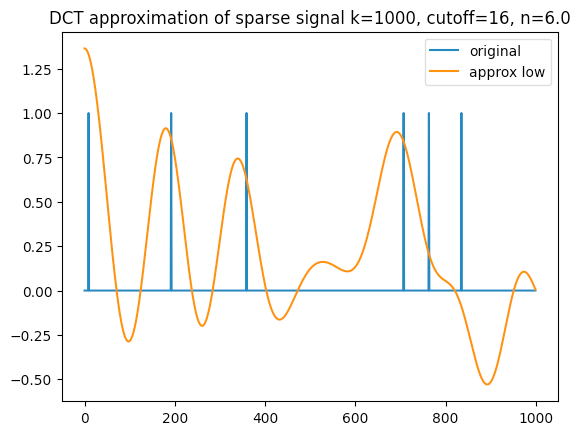
\includegraphics[width=0.7\textwidth]{figures/label-dct-sparse.png}
    \caption{DCT of the label-space using the first 16 components.}
    \label{fig:label-dct-sparse}
\end{figure}

Our second approach uses singular value decomposition (SVD) to compute a projection of label-space into the first few eigenvectors. 
We learn a regression between the features and each of the dimensions found by SVD. 
Then, we compute a prediction using nearest neighbors in the projection of the label-space. 
This process is similar to latent semantic indexing (LSI), and allows for our model to take into consideration cooccurrences between labels. 

As of the time of writing, we are still collecting results for the SVD-KNN approach scaled up to the full dataset.

\subsection{K-NN Survey-Species Modeling}

Instead of building a supervised model from features to response, we can build an unsupervised model that considers distances between survey sites to make predictions. 
Species at sites that are close together should intuitively have similar distributions of plants. 
Our project latitude and longitude has a physical representation via euclidean distance, so we can simply compute nearest neighbors between instances of plant occurrences and return a list of the most frequent (or nearest) plants per survey site.

\subsubsection{Locality-sensitive hashing for K-NN construction and prediction}

We use locality-sensitive hashing using random hyperplane projections to compute nearest neighbors \cite{leskovec2020mining}, with a bucket length of 20 and 5 hash tables. 
We perform an approximate nearest neighbor self-join with a cutoff of 50km. 
Each species instance will be paired with another species instance in the chosen radius. 
We can construct several potential networks from our LSH representation: survey-survey, survey-species, and species-species. 
We consider the species-species multi-network using a threshold of 100km quantized into 10km buckets and see that the majority of edges fall within the first 10km at 318M edges.

\begin{table}
    \centering
    \caption{Counts of euclidean distances within 10km}
    \begin{tabular}{|c|c|}
        \hline
        \textbf{Distance (10km)} & \textbf{Count} \\
        \hline
        0.0 & 318,011,094 \\
        10,000.0 & 146,144,208 \\
        20,000.0 & 117,410,260 \\
        30,000.0 & 99,743,946 \\
        40,000.0 & 85,627,662 \\
        50,000.0 & 75,692,624 \\
        60,000.0 & 73,006,062 \\
        70,000.0 & 65,306,260 \\
        80,000.0 & 58,686,854 \\
        90,000.0 & 52,680,442 \\
        100,000.0 & 23,886,432 \\
        \hline
    \end{tabular}
\end{table}

We can predict directly from the network by choosing the top-k results for each survey site. 
We report the best result below, relative to some of the other models on the leaderboard.

\subsubsection{Node2Vec}

We also experiment with building a node embedding as potential features for a simple regression model. 
The purpose of a network embedding is to learn a representation that preserves desirable properties of the network for downstream machine learning tasks. 
Node2vec \cite{grover2016node2vec} learns to preserve properties of nodes using biased random walks. 
Using the K-NN graph, we attempt to learn both a survey-survey and species-species embedding. 
We find that the survey node embedding is intractable, due to the size of the network at 4 million nodes and ~1 billion edges. 
We are able to compute a species node embedding in about 20 minutes.

A survey node embedding would be immediately useful as a feature for the classification task, since it would require no further processing to go from survey site to species. 
To take advantage of the species embeddings, we would need to compute some average of the embedding vectors before passing into a supervised classification model.

\subsection{Neural Network Models}

Due to technical limitations with classical machine learning techniques, we implement the majority of our non-trivial models with neural networks.
We use PyTorch as our deep learning framework and use PyTorch-Lightning to simplify the training and inference process.
We use Petastorm to preprocess and load data into torch.
We use Weights and Biases to log hyperparameters and metrics.

\begin{table}[]
\title{what}
\caption{}
\label{tab:experiments}
\resizebox{\columnwidth}{!}{%
\begin{tabular}{|l|r|r|r|}
\hline
\textbf{model} & \multicolumn{1}{l|}{\textbf{train f1}} & \multicolumn{1}{l|}{\textbf{validation f1}} & \multicolumn{1}{l|}{\textbf{private}} \\ \hline
v24\_rbgir\_dct                  & 0.3  & 0.21 & 0.15 \\ \hline
v24\_rbgir\_modis\_dct           & 0.28 & 0.28 & 0.03 \\ \hline
v24\_rbgir\_modis\_full\_dct     & 0.12 & 0.13 & NA   \\ \hline
v24\_rbgir\_modis\_bio\_dct      & 0.12 & 0.11 & NA   \\ \hline
v24\_rbgir\_modis\_bio\_idct     & 0.12 & 0.14 & NA   \\ \hline
v1-raster2vec\_classifier\_asl   & 0.19 & 0.19 & 0.14 \\ \hline
v2-raster2vec\_classifier\_multi & 0.12 & 0.12 & 0.13 \\ \hline
\end{tabular}%
}
\end{table}

\subsubsection{Geolocation Baseline Modeling}

Our first model is a simple neural network that learns a relationship between the geospatial features and the species labels.
We use a two-layer network with ReLU activation and a multi-label soft margin loss.
The first layer maps the input into a 256-dimensional latent space, and then second layer maps the latent space into the output space.
This is equivalent to binary cross-entropy (BCE) loss for label.
We use the loss function that accepts logits as input for numerical stability, which is necessary to achieve acceptable convergence.
We evaluate the model using the F1-macro score, which is the closest approximation to the F1-micro score used on the leaderboard.

We found that we were able to learn a relationship between the projected latitude and longitude and the species labels.
However, we noticed that while the loss was decreasing between training and validation sets, the validation F1-macro score would reach a peak on the first epoch and then consistently decrease over time.
We suspect that the cross-entropy loss has difficulty with the class imbalance in the dataset, even when given explicit class weights.
We experimented with alternative loss functions that better represent the multi-label classification score used in the competition.
We cannot use the F1-micro score directly as a loss function, since it is not differentiable.
We test three loss functions that are differentiable surrogates for our score: the multi-label asymmetric loss (ASL) \cite{ridnik2021asymmetric}, the Hill loss \cite{zhang2021simple}, and the SigmoidF1 loss \cite{benedict2021sigmoidf1}.
We find that ASL increases the validation F1-macro scores by a wide margin, likely due to the large number of underrepresented classes in the dataset.
While the Hill loss and SigmoidF1 losses report improvements over ASL in various settings, we find that the default hyper-parameters for these losses perform worse than BCE loss.
With more tuning, it's possible that these losses could perform better than ASL, but for the sake of our experimentation, it is sufficient to have a surrogate loss roughly predictive of the F1-macro score.

\subsubsection{Multi-label Classification with Convolutional Neural Networks}

Once we build our baseline model, we experiment with more complex models for the raster and time-series data.
We note that the data are layered and represented as a 3D tensor, which is a natural fit for convolutional neural networks (CNNs).

The first experiment is to build a CNN model on the RGB-NIR satellite imagery.
We create a CNN model that convolves using a 3x3 kernel with padding that keeps the spatial dimensions the same.
We then use a 1x1 convolution to reduce the number of channels from four to one, followed by a linear layer to map the data to a latent space.
Then, like our geolocation baseline model, we map the latent space to the output space.
We apply ReLU activation after each convolutional layer, and apply batch normalization after each convolutional layer to help with numerical stability.

We find that the model is able to improve over the performance of the geolocation baseline model.
However, we find that it is much more difficult to train a reasonable model on the presence-absent dataset due to how quickly the model converges to a local minima.
We experiment with alternative parameterizations of the network, notably replacing the custom CNN with a pre-packaged efficientnetv2 backbone.
This ends up performing poorly, likely due to several of the pre-processing steps that distort the input data.
We also hypothesize that the larger number of parameters lead to sub-optimal convergence since the space of possible solutions is much larger.

We increase the number of channels by incorporating the MODIS landcover and bio-climatic rasters.
There are 13 landcover classes and 19 bio-climatic classes, which we concatenate with the RGB-NIR channels.
First we add the first 13 channels of the landcover raster to the RGB-NIR channels and find that the initial model does not converge appropriately.
We then take layers 9, 10, and 11 from the raster, which correspond to a modern landcover classification scheme.
Other layers correspond to legacy classification schemes and confidence bands, which are likely not useful to our model.
We then add in a few layers from the bio-climatic rasters, in particular from 2001, 2010, and 2019.
We choose these three bands since they are evenly spaced across the entire set.
We find little improvement over the RGB-NIR and landcover model, possibly due to limiting returns on the number of channels.

Finally, we build a model using the provided time-series RGB-SWIR data.
We reuse the same architecture as the satellite imagery data by reshaping the first 64 coefficients of the time-series DCT into a 8x8 tensor and then applying the same convolutional layers.
The semantics are not necessarily the same as the 2D-DCT coefficients, but we should learn some structure from the basis despite the lack of spatial symmetry.
We find that we learn a model that has predictive power, but it is not as strong as the the baseline geolocation model nor the RGB-NIR model.

\subsubsection{Tile2Vec}

We also experiment with Tile2Vec \cite{jean2019tile2vec}, a self-supervised learning technique that learns embeddings of tiles of satellite imagery.
The Tile2Vec model utilizes a sampling procedure on spatially distributed data and a triplet loss to learn a low dimensional embedding of the data that preserves metric distances via the triangle inequality.
The triplet loss is $L(t_a, t_n, t_d)$ with a margin $m$ where $f_{\theta}$ maps data to a $d$-dimensional vector of real numbers using a model with parameters $\theta$. 

\begin{equation}
    L(t_a, t_n, t_d) = \left[
        ||f_{\theta}(t_a) - f_{\theta}(t_n)||_2
        - ||f_{\theta}(t_a) - f_{\theta}(t_d)||_2
        +m
    \right]_+
\end{equation}

We obtain triplets from the presence-only datasets by sampling one million pairs of tiles that are within 100km of each other using the LSH K-NN graph we constructed earlier.
For each batch of 500 pairs, we randomly choose a distant neighbor from the batch to form the triplet.

We train a tile2vec model using the triplet loss and our basic CNN architecture with a 256-dimensional latent space using the RGB-NIR data.
We find that the model is able to learn a representation of the data that helps with convergence of a downstream classifier.
The classifier is trained by simply adding a linear layer to the learned latent space and training with the ASL loss on the presence-absent dataset.
We note that convergence occurs within four epochs, and that the increase in the F1 metric for both validation and training sets increases monotonically.
In contrast, the models without the tile2vec backbone has validation F1 scores that fluctuate for some time (typically within the first 5 epochs) and then decrease over time.
This suggests a useful intermediate representation can be learned from the more extensive set of loosely labeled data.
However, we note that the learned predictions are marginally less effective than learning the CNN model directly on the presence-absent dataset.

We also experiment with a multi-objective loss incorporating the triplet and ASL losses.
We obtain labels for each survey site by aggregating all species within each site's radius.
Our loss is now simply the sum of the triplet loss with the sum of the ASL loss for each tile.
We found that the triplet loss term no longer decreased monotonically over time.
Instead, it sharply decreased to a minimal, marginally increased, and decreased slowly over time.
The behavior is likely due to the difference in magnitude of the triplet loss and the ASL loss.
The triplet loss is normalized, while the ASL loss is not, so the ASL hyper-parameter dominates the gradient updates.
We could have also used a weighted average of the two losses using a hyperparameter so that we could minimize the overall loss for our specific dataset.
However, the sum of the losses is sufficient to observe relevant behavior.
We find that this version of the model performs better on the transfer learning task to present absent data than the triplet loss alone.

\section{Discussion}

We find difficulty overcoming basic baselines in the competition.
In particular, the frequency-based baseline submissions can be significantly more effective than solutions proposed in our research of the problem.
These solutions are done by predicting the top 25 species at varying levels of locality (e.g. globally or regionally) and by dataset.
However, we find that latitude and longitude are suprisingly predictive of plant species in the dataset given an appropriate loss function.
Using these geospatial features provides a useful diagnostic for more complex datasets, since the number of input features are small and are easier to debug.

\section{Future Work}

We have explored a variety of techniques for finding useful representations of the data to model species distribution.
One area for future work is to better capture nuance associated with the self-supervised representation learning of the tiles.
We quickly reached a limit in how well the model could represent our training data, so it would be useful to rigorously explore alternative model parameterizations and hyperparameters for the various loss functions.
Additionally, it is unclear how to best incorporate the many raster layers that are provided to us in the competition.
Ideally we would be able to determine which layers are most important to the multi-label classification task, possibly through extensive ablation tesing of the features.

We would also like to continue down network or graph models of the survey and species.
There is a rich interconnection between sites and species where sparse co-occurances could be exploited through spatial locality.
One way this could be done is through the construction of node features through message passing of survey site nearest neighbors.
Graph neural networks could also prove to be an effective mechanism to generate useful embedding spaces by propagating information via diffusion.
However, implementation of these techniques could prove to be challenging, especially since we failed to generate a survey embedding through the survey-species bipartite network due to computational constraints.

Our findings indicate a significant variation in the occurrence of the labels, with some labels with less than 10 datapoints while others with more than 10,000. Thus, this cause bias, and imbalance in the training. A possible solution would be to bin the labels according to their frequency, so that each label is relatively in the same range in terms datapoints. This would also potentially allow us to utilize XGBoost, since it would reduce the number of classes needed to be classify.

It would also be interesting to implement a proper model of the dynamics of the remote sensing data.
We are able to build a useful spatial representation of satellite imagery, demonstrated by our experiments with tile2vec.
It should be possible to model the linearized dynamics of a system by learning a Koopman operator that steps forward state-space from one timestep to another.
We hypothesize that this could be done by conditioning the tile embeddings on evolutions of the state e.g. the 20 years of bio-climatic rasters and quarterly time series data.
One potential way to do this is to learn a spatio-temporal embedding of the tiles via an explicit sequence model like a LSTM or transformer alongside methods to enforce the geographical distributional semantics afforded by tile embeddings.
Another approach is to perform data-driven system identification to understand the dynamics of the bio-climatic rasters that have been embedded into the space, and to understand the governing equations of the system with a method like SINDy \cite{brunton2016discovering}.

\section{Conclusions}

In this study, we addressed the multi-label classification challenge of GeoLifeCLEF 2024, which aims to predict the presence or absence of plant species at specific locations based on spatial and temporal remote sensing data. 
We explored various methods for pre-processing the provided datasets and experimented with multiple modeling approaches to tackle the inherent computational challenges and the sparse label space.

\section*{Acknowledgements}

Thank you to Professor Patricio Vela for supervising the project for Anthony Miyaguchi's ECE8903 Special Problems course at Georgia Tech.
Also thank you to the DS@GT CLEF group for their support.

\bibliography{main}

% \appendix
% \section{Online Resources}

\end{document}